\section{Lösung und Konzepte}\label{sec:02_03_loesung_konzept}
\subsection{Standard Aufbau eines Crawlers}
\begin{wrapfigure}{R}{0.4\textwidth}
  \centering
    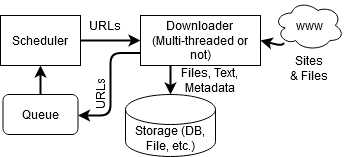
\includegraphics[width=0.4\textwidth]{images/02-Crawler/Crawler-Standard-Crawler.png}
  \caption{\label{fig:standardCrawler}Crawler: Standard Aufbau}
\end{wrapfigure}
Ein Crawler besteht in der Regel aus zwei wichtigen Teilen, einem Downloader und einem Scheduler. Der Downloader ist mit dem Webserver verbunden und lädt die Webseite(n) sowie alle erwünschten Dateien herunter. Der Scheduler ist, wie der Name schon sagt, für die Planung zuständig und erteilt den Tasks des Downloaders URLs, welches nach internen Priorisierung-Mechanismen festgelegt wird. (als Liste FIFO und als Graph mit DFS und BFS ~\cite{ThomasAlgorithms2009}--\cite{DonaldKnuth1998}). 
\subsection{Crawler Mechanismus}
In dem erstellten Projekt werden die Aufgaben des Schedulers vom Crawl-Manager übernommen, welcher sowohl für die Planung als auch für die Steuerung (Start, Pause, Stopp, Zustand) laufender Crawl-Aufgaben zuständig ist. Der Crawl-Manager erzeugt für jede URL ein Thread, einen sogenannten Page-Crawler, dessen Aufgabe darin besteht die Seite herunterzuladen, die Webseite mit dem Page-Analyser auf relevante Daten, wie URLs, Dateien und Links zu prüfen und bei Bedarf weitere parallele Sub-Threads zu erstellen. Diese Sub-Threads sind dann wiederum für den Download, das Parsen und die Speicherung der relevanten Informationen, wie Protokolle, Stammdaten und weiteren Metadaten zuständig. Dieser Mechanismus wird durch die Abb.~\ref{fig:funktionsprinzipCrawler} und die Abb.~\ref{fig:crawlEinerUrl} veranschaulicht.

\begin{figure}[H]
    \centering
    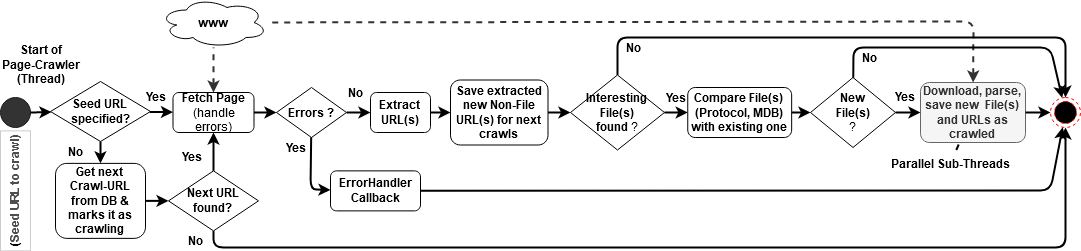
\includegraphics[width=5.5in]{images/02-Crawler/Crawler-Process-Diagram (Page-Crawler).png}
    \caption{Page-Crawler für eine URL}
    \label{fig:crawlEinerUrl}
\end{figure}

\begin{figure}[H]
    \centering
    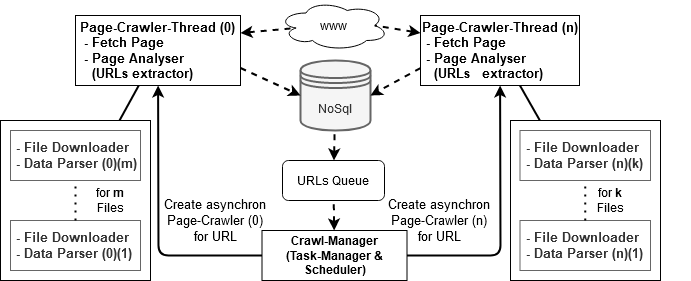
\includegraphics[width=5in]{images/02-Crawler/Crawler-Process-Diagram (Multithreading).png}
    \caption{Funktionsprinzip des unseres Crawlers}
    \label{fig:funktionsprinzipCrawler}
\end{figure}


\noindent
Ein Crawl auf einer Seite, welche durch den Page-Crawler erfolgt, kann in einer durch den Scheduler bzw. Crawl-Manager regelmäßig gemacht werden, in dem dieser nach einer bestimmten Zeit einen neuen Page-Crawl-Thread startet. Die Frequenz der Generierung dieses Threads orientiert sich an dem Sitzungskalender des Bundestags~\cite{Sitzungskalender2021}. Dieser Kalender sieht vor, dass Sitzungen an bestimmten Wochentagen jeweils zwei bis vier Wochen pro Monat stattfinden. Hiervon ausgenommen ist der August aufgrund der Ferienzeit. Darauf basierend ist die Entscheidung getroffen worden, die Frequenz auf einmal pro Tag von Montag bis Freitag festzulegen. Wobei das Stoppen des Crawlers jederzeit manuell möglich ist, wie zum Beispiel innerhalb der Ferien. So lässt sich eine Sperrung wegen zu häufiger Abfragen verhindern. Bei einigen Servern kann es jedoch vorkommen, dass durch bestimmte Serverregeln oder durch den Server-Admin ein sich wiederholendes Abfrage-Muster, zu einer Sperrung der IP-Adresse führen kann. Aus diesem Grund wird zusätzlich zur Frequenz ein Zufallsfaktor verwendet. Ein Page-Crawl-Thread wird von Montag bis Freitag jeweils um 23 Uhr durch den Crawl-Manager gestartet, allerdings wartet dieser Thread eine zufällige Zeit $t$ (mit $10 \leq t \leq 7200 $) bis der tatsächliche Crawl durchgeführt wird. Während und nach dem Crawl-Prozess werden Daten manipuliert, analysiert und gespeichert. Diese Vorgänge sowie die dafür verwendeten Datenstrukturen werden im nächsten Abschnitt näher erläutert. 

\subsection{Daten-Parser und Database-Modell}

Für die Verwendung der vom Crawler heruntergeladenen Plenarprotokolle und Stammdaten müssen diese zunächst in verwendbare Daten umgewandelt werden. Dies übernimmt ein sogenannter Parser, welcher die brauchbaren Informationen aus den Dokumenten ausliest und diese in ein Modell integriert, welches in einer NoSQL-Datenbank gespeichert wird. Um zu verstehen wie der Parser funktioniert und welche Daten relevant sind, muss zuallererst die Datenstruktur der Protokolle und Stammdaten analyisert werden, um auf dessen Basis das bereits genannte Modell zu entwickeln.
\\Im folgenden Abschnitt wird näher auf die Struktur der genannten Dateien eingegangen.
In der Abbildung 2.4 ist die Datenstruktur der Stammdaten zu erkennen. In den Stammdaten stehen jegliche Informationen aller Abgeordneten, welche jemals teil des Bundestages waren. Im folgenden wird stichpunktartig auf die Einzelnen XML-Tags eingegangen:
\begin{itemize}
    \item \textbf{MDB:}  Das Stammdaten-Dokument besteht aus einer Liste dieses Tags, welche den Abgeordneten darstellt
    \item \textbf{ID:} Einzigartige Identifikationsnummer über welche der Abgeordnete in anderen Kontexten referenziert werden kann
    \item  \textbf{NAMEN:} Stellt eine Liste von Namens-Objekten dar, welche mehr als einmal vorhanden sein können, falls sich Änderungen im Namen ergeben haben (z.B. durch eine Heirat)
    \item \textbf{NAME:} Enthält Informationen über den Vor-/Nachnamen, ggf. Präfixe, Titel, wann die Änderung des Namens eingetreten ist, falls es eine gab, etc.
    \item \textbf{WAHLPERIODEN:} Stellt eine Liste von Wahlperioden-Objekten dar, welche angeben in welchen Wahlperioden der Abgeordnete gewählt worden ist
    \item \textbf{WAHLPERIODE:} Enthält Informationen über die Wahlperiode in welcher der Abgeordnete tätig war. Dazu gehören Informationen wie die jeweilige Wahlperiode, Anfang und Ende der Periode, Wahlkreisland und -nummer, als auch die Mandatsart und Daten zur Institution.
    \item \textbf{INSTITUTIONEN:} Stellt eine Liste von Institutions-Objekten dar, welche mehrmals vorhanden sein können, falls der Abgeordnete seine Institution innerhalb der Wahlperiode geändert haben sollte
    \item \textbf{INSTITUTION:} Enthält Daten zur Institution, welche der Abgeordnete zur jeweiligen Wahlperiode angehörte. Dazu gehören Informationen wie Name der Institution (meist der Fraktionsname), Eintritts- und Austrittsdatum, etc.  
    \item \textbf{BIOGRAFISCHE DATEN:} Enthält viele Daten über den Abgeordneten und dessen Leben, wie Geburtsland, -ort, datum, Sterbedatum, Religion, Beruf, Familienstand, Geschlecht, etc.
\end{itemize}

\begin{figure}[H]
    \centering
    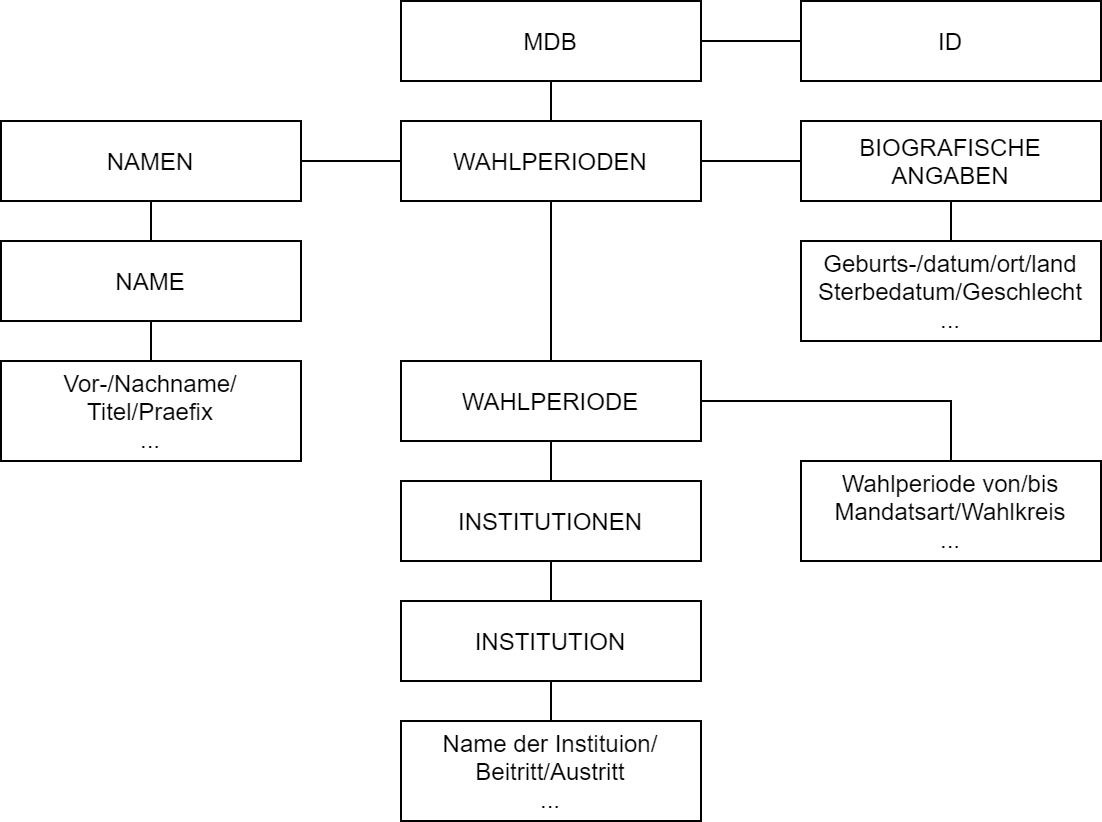
\includegraphics[width=3.5in]{images/02-Crawler/stammdaten_struktur.png}
    \caption{Stammdaten Struktur}
    \label{fig:stammdatenStruktur}
\end{figure}

Aus den vielen Daten der Stammdaten über die Abgeordneten lassen sich unter Umständen einige Erkenntnisse in den späteren Sentimentanalysen verwerten. Für weitere Informationen zur Struktur der Stammdaten kann die DTD-Datei auf der Bundestagsseite eingesehen werden.\\ \\
Die Plenarprotokolle der 19. Legislaturperiode sind ebenfalls im XML Format verfasst, bei welchen die Datenstruktur übersichtlich dargestellt werden kann. Im folgenden wird auf die Struktur des Plenarprotokolls eingegangen. Bei der in Abbildung 2.5 aufgeführten Struktur handelt es sich um eine grob dargestellte Variante, welche nur die für den Parser und somit für das Projekt interessanten Daten aufzeigt. Somit wird im folgenden Abschnitt nicht auf die XML-Tags 'vorspann' und 'anlagen' eingegangen.\\
\begin{itemize}
    \item \textbf{dbtplenarprotokoll:} Enthält alle Informationen über die Bundestagssitzung
    \item \textbf{rednerliste:} Enthält alle Redner, welche in der Sitzung, zu welcher das Protokoll gehört, eine Rede gehalten haben.
    \item \textbf{redner <id>:} Beschreibt den Redner und enthält grobe Informationen über diesen. Zeigt ebenfalls die zugehörige einzigartige ID des Redners, welche in den Stammdaten aufgeführt ist
    \item \textbf{redner/name:} Enthält Informationen wie Vor-, Nachname, Titel und die Fraktion des Abgeordneten
    \item \textbf{sitzungsverlauf:} Enthält alle protokollierten Informationen der Sitzung. Dazu gehören alle angesprochenen Punkte, Reden und Kommentare der teilnehmenden Abgeordneten
    \item \textbf{sitzungsbeginn:} Beginn der Sitzung, welche meist von dem Bundespräsidenten eingeleitet wird. 
    \item \textbf{tagesordnungspunkt:} Informationen über den jeweiligen Tagesordnungspunkt. Unter diesem werden jeweils mehrere Reden von Abgeordneten gehalten auf welche Kommentare und Reaktionen folgen können
    \item \textbf{rede <id>:} Die jeweilige Rede eines Abgeordneten, dessen Inhalt und Reaktionen. Des Weiteren besitzt jede Rede eine chronologische ID, welche nur innerhalb des Protokolls einzigartig ist
    \item \textbf{p:} Dieser Tag stellt einen Paragraphen dar, wobei dessen Inhalt eine Aufnahme der gesagten Worte des jeweiligen Redners darstellen 
    \item \textbf{p <klasse='redner'>:} Dieser Tag mit der Klasse 'redner' ist der erste Paragraph einer Rede und stellt den Redner dar, welcher die Rede führt. Der Redner wird mit groben Informationen und seiner Identifikationsnummer näher beschrieben
    \item \textbf{kommentar:} Kommentar eines Abgeordneten oder einer Fraktion, welches meist aufgrund einer Rede hervorgerufen wird. Dies können Tätigkeiten, wie Beifall oder Zurufe sein.
    \item \textbf{name:} Der Inhalt dieses Tags ist ein einfacher Name desjenigen, welcher innerhalb oder auch außerhalb einer Rede anfängt etwas zu sagen. Anders als ein aufgeführter Redner, führt diese Person meist nur einen kleinen Redeanteil, welcher nicht als eigenständige Rede aufgefasst wird. Ein Beispiel dafür wären die Worte des Bundespräsidenten zur Einleitung der Tagesordnungspunkte. 
\end{itemize}

\begin{figure}[H]
    \centering
    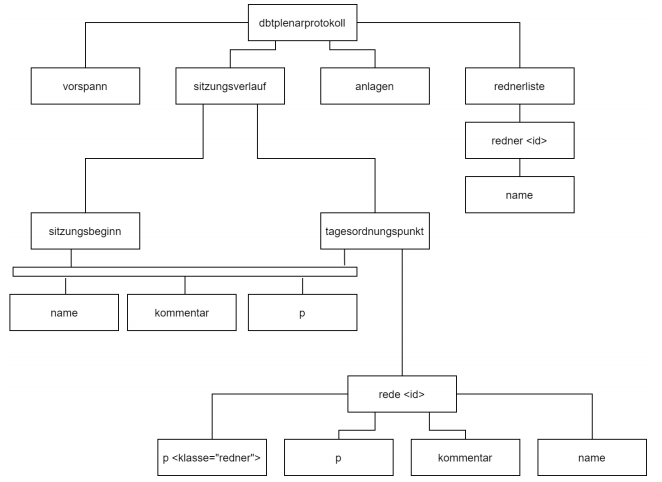
\includegraphics[width=4in]{images/02-Crawler/plenarptokoll_struktur.PNG}
    \caption{Plenarprotokoll Struktur}
    \label{fig:plenarprotokollStruktur}
\end{figure}

Aus der Analyse der beiden Strukturen wurde das Datenbankmodell, welches in Abbildung 2.6 abgebildet ist, erstellt.

\begin{figure}[H]
    \centering
    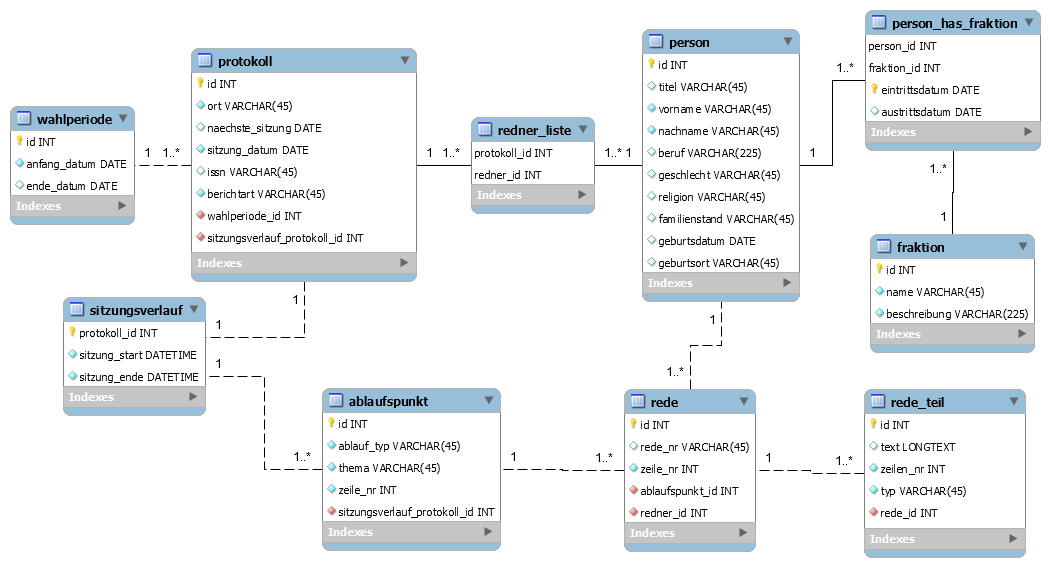
\includegraphics[width=5in]{images/02-Crawler/db_model_bild.png}
    \caption{Datenbankmodell}
    \label{fig:datenbankmodell}
\end{figure}

In diesem Abschnitt wird nur kurz auf das vorliegende Datenbankmodell eingegangen, da die meisten Tabellen und Spalten selbsterklärend sind.
Die Spalte 'id' beschreibt in der Tabelle 'wahlperiode' die jeweilige Legislaturperiode, so wie in der Tabelle 'protokoll' die Sitzungsnummer. Die gesammelten Informationen über die Abgeordneten aus den Stammdaten werden in der Tabelle 'person' gespeichert. Des Weiteren werden deren Fraktionszugehörigkeit, als auch gegebenenfalls Wechsel dieser mit aufgenommen. Die gespeicherten Abgeordneten können nun im späteren Verlauf durch die in der Rednerliste der Protokolle abgespeicherten Identifikationsnummern der Redner referenziert werden. Die Tagesordnungspunkte und der Sitzungsbeginn eines Protokolls werden aufgrund ihrer starken Ähnlichkeit zueinander zu einer Tabelle namens 'ablaufspunkt' zusammengefügt. Lediglich über die Spalte 'ablauf\_typ' ist zu erkennen, ob es sich um einen Tagesordnungspunkt oder ein Sitzungsbeginn handelt. Ebenfalls wurden Paragraphen, welche Redeanteile beinhalten, und Kommentare in der Tabelle 'rede\_teil' zusammengefügt, welche ebenfalls über den Eintrag 'typ' unterschieden werden können. Die Spalte 'paragrafKlasse' in der eben genannten Tabelle gib die 'klasse' des XML-Tags 'p' wieder. Ein Beispiel dazu wäre die in der Protokoll Struktur genannte Darstellung eines Redners über den XML-Tag 'p<klasse='redner'> innerhalb des Protokolls. Die Klasse des Paragraphen beschreibt diesen teils näher. Diese Eigenschaft wurde der Tabelle hinzugefügt aufgrund einer potenziell besseren Verarbeitung der Daten zum Erstellen des Kommunikationsmodells. Des Weiteren werden jeweils die Zeilennummern mitgespeichert, um eine chronologische Reihenfolge der Kommunikationsstruktur zu erhalten.\\
Wie in der Einführung erwähnt müssen die Daten aus den Protokollen mithilfe eines Parsers in ein Modell umgewandelt werden, welches anschließend in der Datenbank gespeichert werden kann. Der Parser dieses Projektes wurde in Java mithilfe des 'Java DOM Parsers' aus der 'JavaX' Bibliothek umgesetzt. Mittels des Parsers wird das XML-Dokument in ein 'Document Object Model' (DOM) umgewandelt. Über die jeweiligen XML-Tags kann dann auf den Inhalt dieser zugegriffen werden. Des Weiteren werden alle XML-Dokumente vor dem Parsen formatiert. Dies ist eine Erweiterung, welche nach einem Problem hinzugefügt worden ist. Aufgrund eines Protokolls, welches vom Ersteller nicht richtig formatiert worden war, kam es zu Problemen der Zeilennummern, da mehrere Tags und somit Inhalte, in einer einzigen Zeile geschrieben worden waren, welches dazu führte, dass keine chronologische Reihenfolge der Kommunikationsstruktur mehr nachvollziehbar war.
Abschließend ist zu erwähnen, dass der Parser nur für die Protokolle und XML-Struktur der 19.Legislaturperiode ausgelegt ist. Wie jedoch bereits in diesem Dokument erwähnt, wird parallel zu diesem Projekt an einer Lösung gearbeitet, welches die Protokolle der 18.Legislaturperiode mithilfe einer KI in die selbe XML-Struktur formatiert. Nach einem Erfolg des eben genannten Projektes wird es ebenfalls möglich sein die 18. Periode zu parsen und diese für weitere Analysen zu verwenden.


\subsection{Gesamter Aufbau der Lösung}
Die gesamte Lösung besteht aus vier Komponenten und einer Datenbank, wie in der Abb.~\ref{fig:crawlerKompoenenten} dargestellt. 
\begin{itemize}
    \item \textbf{Crawl-Manager}: Taskmanager und Scheduler
    \item \textbf{Crawl-Utilities}: Liefert die für den Crawl-Prozess nötigen Funktionalitäten (Page-Fetcher, Page-Analyser, Downloader, Data-Parser)
    \item \textbf{DB-Manager}: Verwaltet den Zugriff auf die Datenbank 
    \item \textbf{Rest-ServiceProvider}: Rest-API für die Steuerung des Crawl-Managers und des eingeschränkten Zugriffs auf die DB-Daten
    \item \textbf{Datenbank}: NoSql (MongoDB) Datenbank zur Sicherung der Daten
\end{itemize}

\begin{figure}[H]
    \centering
    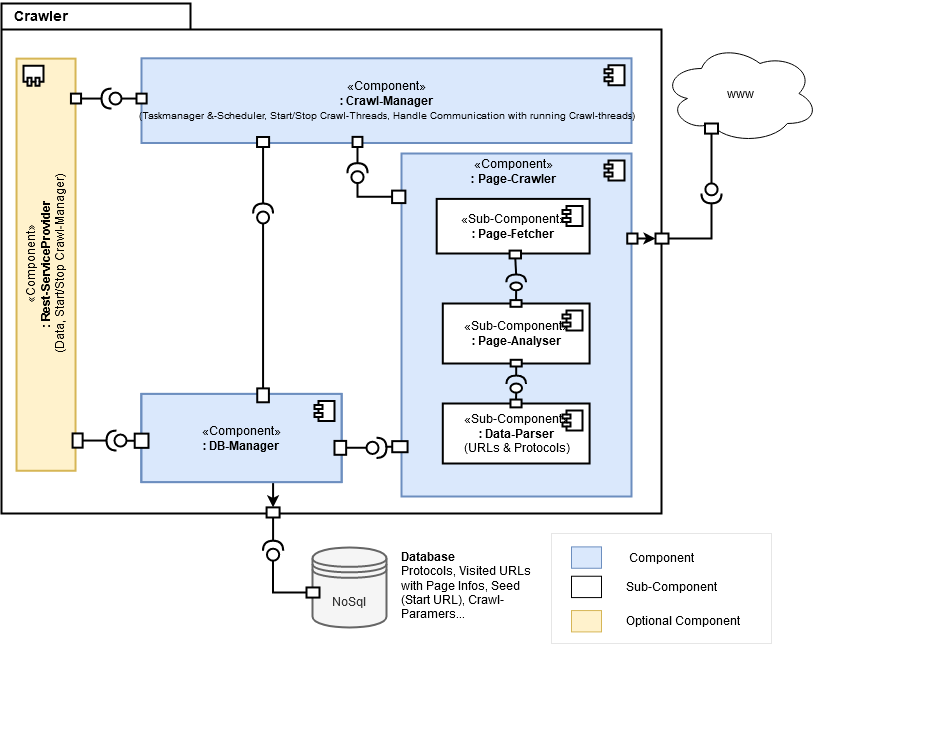
\includegraphics[width=4.3in]{images/02-Crawler/Crawler-Component-Diagram.png}
    \caption{Crawler: Komponentendiagramm}
    \label{fig:crawlerKompoenenten}
\end{figure}
\noindent
Am Ende eines Crawl-Prozesses, bei welchem neue Protokolle oder Stammdaten geladen worden sind, wird die Gruppe des Kommunikationsmodells über eine REST-API~\cite{Cme2021} benachrichtigt. In dieser Benachrichtigung befindet sich eine Liste aller neuen Protokolle sowie Stammdaten, welche als JSON versendet werden. Die Gruppe-Kommunikationsmodell kann im Anschluss asynchron die entsprechenden Dateien aus der bereitgestellten Datenbank laden.